\subsection{Spelling checker \& Slang-Detector}
\textbf{Student Name: }Joelian Samuel \textbf{ ID:} 0872415\\
This subsection describes the spelling checker and slang detector function which were used in raw data preprocessing.
\subsubsection*{Motivation}
A spelling-checking function is needed to increase accuracy when constructing vector for piece of text. Meanwhile, there are some words that will be considered as a typographical error whereas it is a valid word since it is a slang word. Therefore, besides a spelling checking function, the system also needs slang-detector function to check whether a word is categorized as either a typographical error or just a slang word.
\subsubsection*{Problem formulation}
Given a text, the system will try to correct all the mistyped words in that text before passing it to the next process within the pipeline.
\subsubsection*{Approach}
This function was built using Python. We created a class called spellCheck that contains both the spell-checking function and the slang-detector. Figure~\ref{fig:spellprocess}  depicts the process flow from input text unto clean content. 
\begin{figure}
\centering
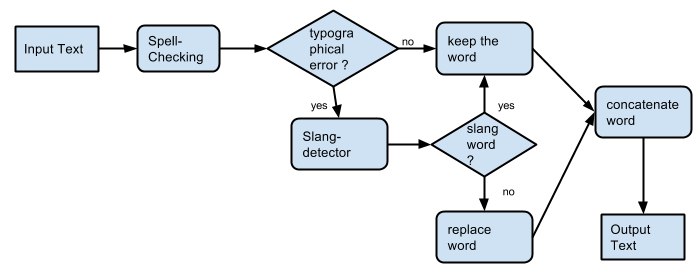
\includegraphics[scale=0.5]{images/spellprocess.png}
\caption{Spelling Checking Process Flow}
\label{fig:spellprocess}
\end{figure}
For the spell-checking and replace-word function, we are using a Python library called PyEnchant. Pyenchant supports many libraries for many languages such as Aspell, Ispell, Myspell, Uspell, Hspell, etc. These libraries are needed to make PyEnchant a generic spell-checking library for many languages. Since, our text will be in English, we only use the Aspell libraries from PyEnchant. Basically, for the spell-checking function, it is boolean retrieval since it will check to find the exact word in dictionary. And for the replacing-word, PyEnchant uses the Levenshtein Distance. Levenshtein Distance is a distance between two string. This distance can be obtained by counting the minimum number of several operations needed to transform one string to another i.e substitution, insertion, deletion of one character, or transposition two adjacent character. \\
For the slang-detector, we are using the API from Urban Dictionary. Besides the common slang word\footnote{taken from Wikipedia : Slang is represented as a lexicon of non-standard words and phrases within a language, typically associated with the subversion of a standard variety} such as ‘lol’, ‘brb’, or ‘lmfao’, this slang-detector also check whether the words is name of product like Samsung, iPhone, or name of places since those kind of words do not appear in the dictionary. Why Urban Dictionary is selected, because it is a dictionary that relies on user contributions. It makes Urban Dictionary becomes the most complete and reliable dictionary for  slang word since slang word can quickly change and increase in term of number. Like spell-checking, this function is also  boolean retrieval.  \\
\subsubsection*{Evaluation}
Given an input text that contains some typographical error  we check the result text to see if the mistake was corrected by the system. Table~\ref{tabelvalspell} shows examples of input and output as produced by our system. From these results we conclude that the function has run correctly.\\ 
\begin{table}[H]
   \resizebox{\textwidth}{!}{
    \begin{tabular}{|l|l}
    \hline
    Input Sentence                                                           & Output sentence                                                      \\ \hline
    Check out the latest PlayStation 4 commercial                            & Check out the latest PlayStation 4  commercial                       \\ \hline
    I say ''I'm always on'' is because I have a sleep disorder i never sleep & I say I m always on is because I have a sleep disorder i never sleep \\ \hline
    \end{tabular}
}
    \caption {Example result of evaluation}
    \label{tabelvalspell}
\end{table}


